\documentclass[12pt,spanish]{article}
% aprovechamiento de la p\'agina -- fill an A4 (210mm x 297mm) page
% Note: 1 inch = 25.4 mm = 72.27 pt
% 1 pt = 3.5 mm (approx)

% vertical page layout -- one inch margin top and bottom
\topmargin      -10 mm   % top margin less 1 inch
\headheight       0 mm   % height of box containing the head
\headsep          0 mm   % space between the head and the body of the page
\textheight     255 mm   % the height of text on the page
\footskip         7 mm   % distance from bottom of body to bottom of foot

% horizontal page layout -- one inch margin each side
\oddsidemargin    0 mm     % inner margin less one inch on odd pages
\evensidemargin   0 mm     % inner margin less one inch on even pages
\textwidth      159 mm     % normal width of text on page

\setlength{\parindent}{0pt}

\usepackage{tikz}
\usetikzlibrary{automata,positioning}

\usepackage[doument]{ragged2e}
\usepackage{babel}
\usepackage[utf8]{inputenc}
\usepackage{amsmath,amsthm,mathtools}
\usepackage{amsfonts,amssymb,latexsym}
\usepackage{enumerate}
\usepackage{subfigure, float, graphicx, caption}
\captionsetup[table]{labelformat=empty}
\captionsetup[figure]{labelformat=empty}
\definecolor{RojoAnayelRey}{rgb}{1,.25,.25}
\usepackage[bookmarks=true,
            bookmarksnumbered=false, % true means bookmarks in 
                                     % left window are numbered                         
            bookmarksopen=false,     % true means only level 1
                                     % are displayed.
            colorlinks=true,
            linkcolor=webred]{hyperref}
\definecolor{webgreen}{rgb}{0, 0.5, 0} % less intense green
\definecolor{webblue}{rgb}{0, 0, 0.5}  % less intense blue
\definecolor{webred}{rgb}{0.5, 0, 0}   % less intense red
\definecolor{dkgreen}{rgb}{0,0.6,0}
\definecolor{gray}{rgb}{0.5,0.5,0.5}
\definecolor{mauve}{rgb}{0.58,0,0.82}
\definecolor{MistyRose}{RGB}{255,228,225}
\definecolor{LightCyan}{RGB}{224,255,255}

% \usepackage{beton}
% \usepackage[T1]{fontenc}

% Theorem environments

%% \theoremstyle{plain} %% This is the default
\newtheorem{theorem}{Teorema}[section]
\newtheorem{corollary}[theorem]{Corolario}
\newtheorem{lemma}[theorem]{Lema}
\newtheorem{proposition}[theorem]{Proposici\'on}
%\newtheorem{ax}{Axioma}

\theoremstyle{definition}
\newtheorem{definition}{Definici\'on}[section]
\newtheorem{algorithm}{\textrm{\bf Algoritmo}}[section]

\theoremstyle{remark}
\newtheorem{remark}{Observaci\'on}[section]
\newtheorem{example}{Ejemplo}[section]
\newtheorem{exercise}{Ejercicio}%[section]
%\newenvironment{solution}{\begin{proof}[Solution]}{\end{proof}}
\newenvironment{solution}{\begin{proof}[Solución]}{\end{proof}}
\newtheorem*{notation}{Notaci\'on}

%\numberwithin{equation}{section}

%\newcommand{\regla}[2]{
%\begin{array}{c}
%#1\\
%\hline
%#2\\
%\end{array}
%}
\begin{document}

\title{Modelos de Computación: \\ Relación de problemas 1}
\author{David Cabezas Berrido}
\date{\vspace{-5mm}}
\maketitle

\setcounter{exercise}{16}
\begin{exercise}~ Autómata finito determinista que reconoce el
  lenguaje
  \[L_1=\{u\in\{0,1\}^* \ | \text{ el número de 1's no es múltiplo de 3}\}\] \vspace{-10mm}
  \begin{figure}[H]
  \centering
  \subfigure{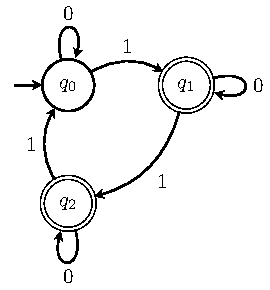
\includegraphics[width=60mm]{17_1}}
\end{figure}
\vspace{-10mm}
  \[L_2=\{u\in\{0,1\}^* \ |\text{ el número de 0's es par}\}\] \vspace{-10mm}
  \begin{figure}[H]
  \centering
  \subfigure{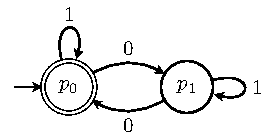
\includegraphics[width=70mm]{17_2}}
  \end{figure} \vspace{-5mm}
  Ahora sólo tenemos que intersecar los dos autómatas para formar el
  deseado, el que reconoce el lenguaje
  \[L_3=\{u\in\{0,1\}^* \ |\text{ el número de 1's no es múltiplo de 3 y el número de 0's es par}\}\]
  \begin{figure}[H]
  \centering
  \subfigure{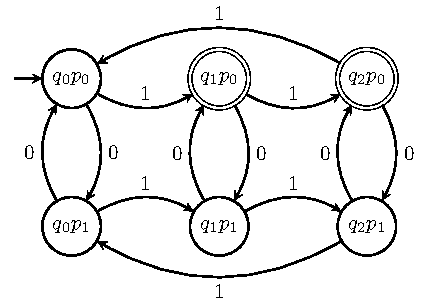
\includegraphics[width=75mm]{17_3}}
  \end{figure}
  
\end{exercise}

\setcounter{exercise}{21}
\begin{exercise}~ Para hallar la expresión regular que representa el lenguaje aceptado por el autómata \vspace{-5mm}
\begin{figure}[H]
  \centering
  \subfigure{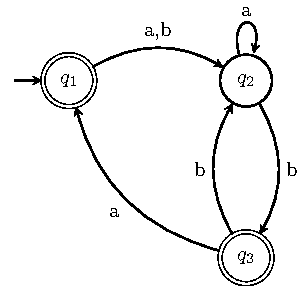
\includegraphics[width=50mm]{22}}
\end{figure} \vspace{-5mm}
usaremos el algoritmo visto en clase (sólo mostraré un par de iteraciones)
\begin{align*}
  r_{11}^3&+r_{13}^3 \\
  r_{11}^2+r_{13}^2(r_{33}^2)^*r_{31}^2&+r_{13}^2+r_{13}^2(r_{33}^2)^*r_{33}^2 \\
  \varepsilon+(a+b)a^*b(a(a+b)a^*b+ba^*b)^*a&+(a+b)a^*b+(a+b)a^*b(a(a+b)a^*b+ba^*b)^+ \\
  \varepsilon+(a+b)a^*b\big(\varepsilon+(a(a+b)a^*b&+ba^*b)^*a+(a(a+b)a^*b+ba^*b)^+\big) \\
  \varepsilon+(a+b)a^*b\big((a(a+b)a^*b&+ba^*b)^*a+(a(a+b)a^*b+ba^*b)^*\big) \\
  \varepsilon+(a+b)a^*b\big((a(a+b)a^*b&+ba^*b)^*(a+\varepsilon)\big)
\end{align*}
\end{exercise}

\begin{exercise}~ Para probar que
  $B_n=\{a^k \ | \text{ k es múltiplo de n}\}=\{a^{kn} \ | \ k \in
  \mathbb{N}\}$ es regular para todo $n$, construiremos un autómata
  finito determinista que lo reconozca.

  $B_0=\{\varepsilon\}$ es trivialmente regular, lo reconoce el autómata \vspace{-5mm}
\begin{figure}[H]
  \centering
  \subfigure{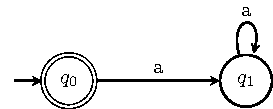
\includegraphics[width=50mm]{23_b0}}
\end{figure} \vspace{-5mm}
$B_1=\{a\}^*$ es reconocido por \vspace{-7mm}
\begin{figure}[H]
  \centering
  \subfigure{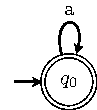
\includegraphics[width=20mm]{23_b1}}
\end{figure}
$B_2=$ palabras sobre $\{a\}^*$ con número par de $a$'s es reconocido por
\begin{figure}[H]
  \centering
  \subfigure{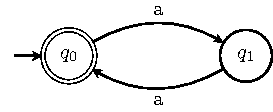
\includegraphics[width=50mm]{23_b2}}
\end{figure}

\newpage

$B_3$ por 
\begin{figure}[H]
  \centering
  \subfigure{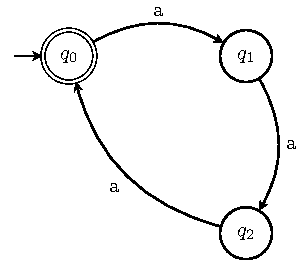
\includegraphics[width=50mm]{23_b3}}
\end{figure}

De esta forma,
$M_n=(\{q_0,\ldots,q_{n-1}\},\{a\},q_0,\delta_n,\{q_0\})$ con
\\ $\delta_n(q_i,a)=q_{(i+1)\%n}$ $\forall i=0,\ldots,n-1$ es un
autómata finito determinista que reconoce el lenguaje $B_n$
$\forall n\geq 2$. \\

También puede razonarse que $B_n=(a_1a_2\ldots a_n)^*$ donde
$a_i=a \ \forall i$.
\end{exercise}

~

\begin{exercise}~ Dado un lenguaje regular $L$, probaremos que los
  siguientes lenguajes son regulares \\
  
  $a) \ NOPREFIJO(L)=\{u\in L \ |$ ningún prefijo propio de $u$ pertenece a $L\}$ \\

  Buscamos eliminar las palabras del lenguaje que tienen prefijos
  propios que pertenecen al lenguaje, podemos conseguir esto con tan
  sólo hacer inaccesibles algunos de los estados finales del autómata.

  Primero lo haré para $\varepsilon \notin L$.
  Supongamos que $M=(Q,A,q_0,\delta,F)$ es un autómata finito
  determinista que reconoce a $L$. Construimos
  $M'=(Q\cup\{p\},A,q_0,\delta',F)$ y definimos $\delta'$ de la
  siguiente forma
  \begin{align*}
    \delta'(f,a)=&p \quad \forall f \in F, \ \forall a \in A \\
    \delta'(p,a)=&p \quad \forall a \in A \\
    \delta'(q,a)=&\delta(q,a) \quad \text{en el resto de casos}
  \end{align*}
  Si $u$ es aceptada por $M'$, significa que $\delta'(q_0,u) \in F$,
  además no hemos pasado por ningún estado final en medio (de haberlo
  hecho acabaría ciclando en $p$), por lo que siempre hemos aplicado
  la definición del resto de casos, esto significa que ningún prefijo
  propio de $u$ es aceptado por $M'$ y que todas las palabras
  aceptadas por $M'$ son de $L$. \\

  En el autómata finito determinista que he hallado, si
  $\varepsilon \in L$, hacemos que $\delta'(q_0,a)=\delta(q_0,a)$
  aunque se trate de un estado final. Creamos un nuevo estado final
  $q_0'$, para el que definimos $\delta'$ como en el resto de estados
  finales y modificamos $\delta'$ para que que si $\delta(q,a)=q_0$,
  entonces $\delta'(q,a)=q_0'$.

  Resumiendo, hemos encontrado un autómata finito determinista que
  reconoce $NOPREFIJO(L)$, luego es regular. \\

$b) \ NOEXTENSION(L)=\{u\in L \ | \ u$ no es prefijo propio de ninguna
palabra de $L\}$ \\

  Si un estado es final pero leyendo más símbolos se puede llegar a
otro (o el mismo) estado final, se deben eliminar del lenguaje las
palabras que lleven a ese estado. Esto lo conseguimos eliminando
estados finales.

Primero lo haré para $\varepsilon \notin L$.
  Supongamos que $M=(Q,A,q_0,\delta,F)$ es un autómata finito
determinista que reconoce a $L$. Construimos $M'=(Q,A,q_0,\delta,F')$
donde
  \[F'=\{q\in F \ | \ \nexists u \in A^+, \ \nexists f \in F :
(q,u)\vdash^* (f,\varepsilon)\}\]

De esta forma, $M'$ sólo acepta palabra de $L$. Además, de toda
palabra $u$ aceptada por $M'$, sabemos que no existe otra palabra $v
\neq \varepsilon$ tal que $uv \in L$ justo como queríamos. \\

  Resumiendo, hemos encontrado un autómata finito determinista que
reconoce $NOEXTENSION(L)$, luego es regular. \\

En el autómata finito determinista que he hallado, si la palabra vacía
está en $L$, se debe eliminar el estado inicial $q_0$ del conjunto de
estados finales y añadir una transición nula de $q_0$ a otro nuevo
estado final $r$. Ahora tengo un autómata finito con transiciones
nulas que reconoce $NOEXTENSION(L)$, luego es regular.
\end{exercise}
~

\begin{exercise}~ $L\subseteq A^*$ define una relación $\equiv$ en
  $A^*$.
  \[u\equiv v \text{ si y sólo si } \forall z\in A^* \text{ se tiene }
    (uz\in L \Leftrightarrow vz \in L)\]

  \begin{enumerate}[a)]
  \item Probemos que $\equiv$ es una relación de equivalencia
    \begin{enumerate}
    \item[Reflexiva:]
      $(uz\in L \Leftrightarrow uz \in L) \ \forall z\in A^*$, luego
      $u\equiv u \ \forall u\in A^*$.
    \item[Simétrica:]
      $(uz\in L \Leftrightarrow vz \in L) \Leftrightarrow (vz\in L
      \Leftrightarrow uz \in L)$, luego
      $u\equiv v \Leftrightarrow v\equiv u$.
    \item[Transitiva:] Si $(uz\in L \Leftrightarrow vz \in L)$ y
      $(vz\in L \Leftrightarrow wz \in L)$ claramente tenemos \\
      $(uz\in L \Leftrightarrow wz \in L)$, luego $u\equiv v$ y
      $v\equiv w$ implica $u\equiv w$.      
    \end{enumerate}

  \item Calcularemos las clases de equivalencia de
    $L=\{a^ib^i|i\geq 0\}$.

    $C=$ Clase de las palabras que no son prefijo de ninguna palabra
    de $L$:
    \begin{itemize}
    \item Palabras de la forma $A^*bA^*aA^*$.
    \item Palabras de la forma $a^ib^j$ donde $j>i\geq 0$.
    \end{itemize}
    
    $C_{ij}$ ($i \geq j \geq 0$) = Clase de equivalencia de la
    palabra $a^ib^j$ (formada únicamente por dicha palabra).

  \item Calcularemos las clases de equivalencia de
    $L=\{a^ib^j|i,j\geq 0\}$.

    $C=$ Clase de las palabras que no son prefijo de ninguna palabra
    de $L$, son de la forma $A^*bA^*aA^*$.
    
    $C_a=$ Clase de equivalencia de las palabras de la forma $a^i$ con
    $i\geq 0$.

    $C_b=$ Clase de equivalencia de las palabras de la forma $a^ib^j$
    con $i\geq 0, \ j>0$.

  \item Probaré que $L$ es aceptado por un autómata finito
    determinista si y sólo si el número de clases de equivalencia es
    finito.

    Si $L$ es aceptado por un autómata finito determinista, debe
    existir un autómata minimal que lo acepte (obviamente finito), en
    el apartado siguiente pruebo que palabras de distinta clase de
    equivalencia llevan a estados distintos, luego el número de clases
    de equivalencia debe ser finito.

    Si el número de clases de equivalencia de $L$ es finito
    ($C_0,\ldots,C_{n-1}$, podemos suponer $\varepsilon \in C_0$),
    creamos un autómata que lo reconozca:
    $M=(\{q_0,\ldots,q_{n-1}\},A,q_0,\delta,F)$
    \begin{align*}
      \delta(q_i,a)=&q_j \text{ donde $C_j$ es la clase de equivalencia de $u_ia$, siendo $u_i$ cualquier palabra de $C_i$}\\
      F=&\{q_i \in Q | u \in C_i \implies u \in L\}
    \end{align*}

    Tanto $\delta$ como $F$ están bien definidos, ya que el
    representante de la clase es arbitrario. En la definición de $F$,
    si $v$ es otra palabra de $C_i$,
    $u\varepsilon \in L \Rightarrow v = v\varepsilon \in L$.

    En la definición de $\delta$, si $v_i$ es una palabra de la misma
    clase de equivalencia $C_i$, la clase de $v_ia$ será la misma que
    la de $u_ia$. Demostración: dado $z \in A^*$ cualquiera
    \[(v_ia)z \in L \Leftrightarrow v_i(az) \in L \Leftrightarrow
      u_i(az) \in L \Leftrightarrow (u_ia)z \in L\]

    Probemos que $M$ efectivamente reconoce el lenguaje $L$:

    Si $u \in A^*$ es aceptada por $M$, la clase de $u$ (supondremos
    $C_i$ se corresponderá con un estado final de $M$ ($q_i$). Pero
    los estados finales son los que cumplen que cualquier
    representante pertenece al lenguaje, luego $u \in L$.

    Si $u \in L$, $\delta(q_0,u)$ corresponderá a una clase de
    equivalencia asociada a un estado final (ya que tiene un
    representante que pertenece al lenguaje), luego $M$ aceptará $u$.

  \item La relación que existe entre el número de clases de
    equivalencia y el autómata finito minimal que acepta $L$ es que el
    número de clases de equivalencia es el número de estados del
    autómata.

    La idea es que si $u$ y $v$ son dos palabras de la misma clase de
    equivalencia, $q_u=\delta(q_0,u)$ y $q_v=\delta(q_0,v)$ deben ser
    el mismo estado, ya que $\forall z \in A^*$ tenemos que
    $\delta(q_u,z) \in F \Leftrightarrow \delta(q_v,z) \in F$ y si
    $q_u \neq q_v$ se podrían unificar, contradiciendo así la
    propiedad de ser minimal.

    Recíprocamente, si $u$ y $v$ no pertenecen a la misma clase de
    equivalencia $q_u$ y $q_v$ deberán ser diferentes, ya que existe
    un $z\in A^*$ cumpliendo $\delta(q_u,z) \in F$ y
    $\delta(q_v,z) \notin F$ o viceversa.
  \end{enumerate}
  
\end{exercise}

\end{document}
